\section{Integrieren wie Cauchy}

\begin{karte}{Integrale der Form \( \int_{-\infty}^\infty \frac{P(x)}{Q(x)} \dx{x} \) Teil 1}
    \(Q(x) \neq 0\) für alle \(x\in \R \Rightarrow \int_{-R}^R \frac{P(x)}{Q(x)} \dx{x}\) 
    existiert für alle \(R>0\). \\
    Falls \(\deg Q \geq \deg P+2\). Dann konvergieren 
    \[ \int_0^R \frac{P(x)}{Q(x)} \dx{x} \text{ und } \int_{-R}^0 \frac{P(x)}{Q(x)} \dx{x} \]
    im Grenzwert \(R \rightarrow \infty\) und somit ist dann 
    \[ \int_{-\infty}^\infty \frac{P(x)}{Q(x)} \dx{x} = \limes{R} \int_{-R}^R \frac{P(x)}{Q(x)} \dx{x}. \]
    \begin{center}
        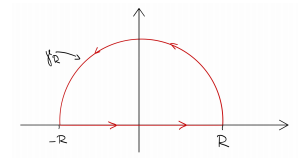
\includegraphics[width=0.4\textwidth]{img/kurve-halbebene.png}
    \end{center}
\end{karte}

\begin{karte}{Integrale der Form \( \int_{-\infty}^\infty \frac{P(x)}{Q(x)} \dx{x} \) Teil 2}
    Aus dem Residuensatz folgt 
    \[ \int_{\gamma_R} \frac{P(z)}{Q(z)} \dx{z} = 2\pi i \sum_k \Res(\frac{P}{Q}, z_k), \]
    wobei die \(z_k\) die Nullstellen von \(Q\) in \(C_+\) sind, die im 
    Inneren von \(\gamma_R\) liegen, sind. Sofern \(R\) groß genug ist, 
    geht dies über alle Nullstellen von \(Q\) in der oberen Halbebene.
    \[ \Rightarrow \int_{-R}^R \frac{P(x)}{Q(x)} \dx{x} + \int_{\Gamma_R} \frac{P(z)}{Q(z)} \dx{z} = 2\pi i \sum_k \Res(\frac{P}{Q}, z_k), \]
    wobei \(\Gamma_R := \set{z\in \C_+: \abs{z} = R} = \set{z: \Im z > 0, \abs{z} = R}\) 
    der obere Halbkreis vom Radius \(R\) ist.\\
    Zu zeigen \( \limes{R} \int_{\Gamma_R} \frac{P(z)}{Q(z)} \dx{z} = 0 \). (\(ML\)-Formel) 
    Dann folgt 
    \[ \int_{-\infty}^\infty \frac{P(x)}{Q(x)} \dx{x} = 
    \limes{R} \int_{-R}^R \frac{P(x)}{Q(x)} \dx{x} 
    = 2\pi i \sum_k \Res(\frac{P}{Q}, z_k). \]
\end{karte}

\begin{karte}{Integrale der Form \(\int_{-\infty}^\infty R(x) \cos(bx) \dx{x}\) (oder mit \(\sin\))}
    Sei \(R(\frac{x}{b}) = \frac{P(x)}{Q(x)}, Q(x) \neq 0\) außer in den Nullstellen von \(\cos(bx)\)
    und \(\sin(bx)\). Sofern \(\deg P \geq \deg Q + 1\), konvergieren die Integrale.
    Wir behaupten für \(b>0\): 
    \[ \limes{R} \int_{\Gamma_R} R(z) e^{ibz} \dx{z} = 0 \]
    und dann auch 
    \[ \int_{-\infty}^\infty R(x) e^{ibx} \dx{x} = \limes{R} \int_{\gamma_R} R(z) e^{ibz} \dx{z} \]
    und somit haben wir 
    \[ \int_{-\infty}^\infty R(x) \cos(bx)\dx{x} = \Re \left[ 2\pi i \sum_k \Res(R(z) e^{ibz}, z_k) \right] \]
    und 
    \[ \int_{-\infty}^\infty R(x) \sin(bx)\dx{x} = \Im \left[ 2\pi i \sum_k \Res(R(z) e^{ibz}, z_k) \right]. \]
    Falls \(b<0\), können wir in der unteren Halbebene \(\C_-\) integrieren.
\end{karte}

\begin{karte}{Trigonometrische Integrale über \([0,2\pi]\)}
    Integrale der Form 
    \[ \int_0^{2\pi} U(\cos \theta, \sin \theta) \dx{\theta} \]
    mit \(U\) rational, also \(U = \frac{P}{Q}\).\\
    Mache Substitution \(z = e^{i\theta}\), dann folgt 
    \(d\theta = \frac{dz}{iz}\).
    \[ \Rightarrow \int_0^{2\pi} U(\cos \theta, \sin \theta) dx{\theta} = \int_{\partial \mathbb{D}} F(z) \dx{z} \]
    mit \(F(z) := U(\frac{1}{2} (z + z^{-1}), \frac{1}{2i} (z - z^{-1}) ) \frac{1}{iz}\).
\end{karte}

\begin{karte}{Integrale der Form \( \int_0^\infty \frac{P(x)}{Q(x)} \dx{x} \) (Schlüssellochwege) \\Teil 1}
    Annahme: \(\deg P \geq \deg Q + 2, Q(x) \neq 0\) für alle \(x\geq 0\). 
    Ist \(\frac{P(x)}{Q(x)}\) gerade (\(f(x) = f(-x)\)), so ist 
    \[ \int_0^\infty \frac{P(x)}{Q(x)} \dx{x} = \int_{-\infty}^0 \frac{P(x)}{Q(x)} \dx{x} = 
    \frac{1}{2} \int_{-\infty}^\infty \frac{P(x)}{Q(x)}\dx{x}. \]
    Ansonsten setze \(R(z) = \frac{P(z)}{Q(z)}\) und betrachte \(R(z) \log z\) auf 
    \(\C \setminus [0,\infty)\).\\
    Ist \(x > 0\) und \(z = xe^{i\theta}\), so ist \(\log z = \log x + i\theta \rightarrow \log x\).
    Wählen wir die Schlüssellochkontur 
    \begin{center}
        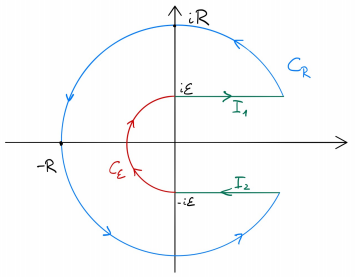
\includegraphics[width=0.4\textwidth]{img/kurve-schluesselloch.png}
    \end{center}
\end{karte}

\begin{karte}{Integrale der Form \( \int_0^\infty \frac{P(x)}{Q(x)} \dx{x} \) (Schlüssellochwege) \\Teil 2}
    \begin{enumerate}
        \item horizontales Liniensegment \(I_1 = I_1(\varepsilon, R)\) von \(i\varepsilon\) 
        zu \(\sqrt{R^2-\varepsilon^2} + i\varepsilon\)
        \item Kreisbogen \(C_R\) (gegen Uhrzeigersinn) von \(\sqrt{R^2-\varepsilon^2} + i\varepsilon\) 
        zu \(\sqrt{R^2-\varepsilon^2} - i\varepsilon\)
        \item horizontales Liniensegment \(I_2 = I_2(\varepsilon, R)\) von 
        \(\sqrt{R^2-\varepsilon^2} - i\varepsilon\) zu \(-i\varepsilon\)
        \item Halbkreis \(C_\varepsilon\) mit Radius \(\varepsilon\) von 
        \(-i\varepsilon\) zu \(i\varepsilon\) (im Uhrzeigersinn)
    \end{enumerate}
    Aus dem Residuensatz folgt 
    \[ \lim_{\varepsilon\rightarrow 0, R \rightarrow \infty} 
    \int_{K_{\varepsilon, R}} R(z) \log z \dx{z} 
    = 2\pi i \sum_k \Res(R(z \log z, z_k)), \]
    ist \(\varepsilon\) klein und \(R\) groß genug, so sind alle Nullstellen von 
    \(Q\) im Inneren von \(K_{\varepsilon, R}\).
    \[ \lim_{\varepsilon\searrow 0} \int_{I_1(\varepsilon,R)} R(z) \log z \dx{z} 
    = \int_0^R R(x) \log x \dx{x}. \]
    \[ \lim_{\varepsilon\searrow 0} \int_{I_2(\varepsilon, R)} R(z) \log z \dx{z} 
    = \int_R^0 R(x) (\log x + 2\pi i) \dx{x} = -\int_0^R R(x) (\log(x) + 2\pi i) \dx{x}. \]
\end{karte}

\begin{karte}{Integrale der Form \( \int_0^\infty \frac{P(x)}{Q(x)} \dx{x} \) (Schlüssellochwege) \\Teil 3}
    Also folgt, falls die Integrale über die Kreisteile \(=0\) sind, 
    \[ \int_0^\infty \frac{P(x)}{Q(x)} \dx{x} = -\sum_k \Res(\frac{P(z)}{Q(z)} \log z, z_k), \]
    wobei \(z_k\) die Nullstellen von \(Q\) in \(\C \setminus [0,\infty)\) sind.\\
    Integrale der Form \(\int_a^\infty \frac{P(x)}{Q(x)} \dx{x}\) kann man 
    lösen, indem man 
    \[ \int_{K_{\varepsilon, R}} \frac{P(z)}{Q(z)} \log(z-a) \dx{z} \]
    betrachtet, wobei \(K_{\varepsilon, R}\) jetzt um \(a\) nach rechts verschoben ist.
\end{karte}